\documentclass[draft,grl]{agujournal2018}
%\documentclass[]{agujournal2018}
\usepackage{apacite}
\usepackage{url}
\usepackage{lineno}

%\draftfalse
\journalname{Geophysical Research Letters}

%custom packages
\usepackage{amsmath,amssymb,amsfonts,amsthm}
\usepackage{comment}
\usepackage{booktabs}
% custom commands
\newcommand\be{\begin{equation}}
\newcommand\ee{\end{equation}} 
\newcommand\bra{\langle}
\newcommand\ket{\rangle}
\newcommand\om{\omega}
\newcommand\tom{\tilde{\omega}}
\newcommand\tg{\tilde{g}}
\newcommand\tp{\tilde{p}}
\newcommand\tG{\tilde{G}}
\newcommand\El{\mathcal{L}}
%\usepackage{layouts}
%\printinunitsof{in}\prntlen{\textwidth} % check scales in the document
\linenumbers

% THIS IS THE LINENO PATCH TO WORK WITH AMSMATH
\newcommand*\patchAmsMathEnvironmentForLineno[1]{%
	\expandafter\let\csname old#1\expandafter\endcsname\csname #1\endcsname
	\expandafter\let\csname oldend#1\expandafter\endcsname\csname end#1\endcsname
	\renewenvironment{#1}%
	{\linenomath\csname old#1\endcsname}%
	{\csname oldend#1\endcsname\endlinenomath}}% 
\newcommand*\patchBothAmsMathEnvironmentsForLineno[1]{%
	\patchAmsMathEnvironmentForLineno{#1}%
	\patchAmsMathEnvironmentForLineno{#1*}}%
\AtBeginDocument{%
	\patchBothAmsMathEnvironmentsForLineno{equation}%
	\patchBothAmsMathEnvironmentsForLineno{align}%
	\patchBothAmsMathEnvironmentsForLineno{flalign}%
	\patchBothAmsMathEnvironmentsForLineno{alignat}%
	\patchBothAmsMathEnvironmentsForLineno{gather}%
	\patchBothAmsMathEnvironmentsForLineno{multline}%
}
% the patch comes from http://phaseportrait.blogspot.com/2007/08/lineno-and-amsmath-compatibility.html

\begin{document}

\title{Back to Einstein: how to include burial in fluvial sediment diffusion models?}

\authors{James K. Pierce \affil{1}and Marwan A. Hassan\affil{1}}
\affiliation{1}{Department of Geography \\University of British Columbia}
\correspondingauthor{James Kevin Pierce}{kpierce@alumni.ubc.ca}

\begin{keypoints}
\item We develop a random walk model of objects in intermittent transport through an environment with traps
\item Its solution provides three ranges of diffusion, two of which are anomalous
\item We apply the model to sediment transport in rivers to clarify the scale dependence of bedload diffusion

\end{keypoints}

\begin{abstract}
Sediment grains transport through gravel bed rivers in cycles of motion and rest.
When grains rest on the surface, material transported from upstream can bury them.
The surface shields buried grains from the flow, so they can be immobile for long time periods.
These immobile periods can dominate sediment diffusion characteristics.
Although investigators have recognized the impact of sediment burial on diffusion, existing models do not usually incorporate it.
In this study, we present a random walk model incorporating sediment burial and solve it analytically.
The model predicts three sediment diffusion ranges with distinct scaling characteristics in each.
We relate the crossover times dividing these ranges to measurable transport parameters and describe each range from underlying physical processes.
Our developments provide new geophysical perspective on the scale dependence of fluvial sediment transport.
\end{abstract}

\section{Introduction}

Anomalous diffusion has been subjected to intense research lately, as it emerges in contexts ranging from the transport of cholesterols through lipid bilayers \citep{Jeon2012,Molina-Garcia2018}, to contaminants through soils \citep{Berkowitz2006,Yang2019}, and pollinator insects through ecosystems \citep{Reynolds2009,Vallaeys2017}.
In this paper, we study anomalous diffusion in a river science context, where it emerges from coarse bedload sediment transporting through river channels \citep{Bradley2017,Martin2012,Ganti2010}.
Hans Albert Einstein developed the first model of bedload diffusion to describe his comprehensive experiments visually tracking painted grains through a flume \citep{Ettema2004,Einstein1937}.
Diffusion is the spreading apart of grains as they transport downstream, and it is induced by differences in the transport characteristics of one grain and the next.
Diffusion is usually quantified by the time dependence of the positional variance $\sigma_x^2(t)$ of a population.
With the scaling $\sigma_x^2 \propto t$, the diffusion is said to be normal, since this is found in the classic diffusion problems \citep[e.g.,][]{Einstein1905,Taylor1920}.
However, many transport phenomena show $\sigma_x^2 \propto t^\gamma$ with $\gamma \neq 1$.
This diffusion is said to be anomalous \citep{Sokolov2012}. 
If $\gamma>1$, it is said to be super-diffusive; while if $\gamma <1$, it is said to be sub-diffusive \citep{Metzler2000}.
Einstein originally concluded that bedload transport shows normal diffusion.

After Einstein, \citet{Nikora2001a,Nikora2002} recognized that coarse sediment moving through river channels can show either anomalous or normal diffusion depending on the timescale of observation.
This is a significant issue since it implies diffusion models should be scale dependent, and it renders experimental data contingent on their observation timescales.
Nikora et al. identified three ranges of diffusion from Newtonian simulations and experimental data and termed these ranges local, intermediate, and global in order of increasing timescale.
They determined that $\sigma_x^2$ scales with a different power of time in each range, and they concluded this scaling could be anomalous or normal.
Recent studies support the Nikora et al. conclusion that bedload diffusion is scale dependent, but they do not show consensus on the details of their three range concept.
For example, various numerical approaches show two \citep[e.g.,][]{Fan2016} or three \citep[e.g.,][]{Bialik2012,Zhang2012} ranges of diffusion; one set of flume experiments shows two ranges of sediment diffusion \citep{Martin2012}, and two field studies show anomalous diffusion \citep{Bradley2017, Phillips2013}; but taken together, these studies leave us unclear on the expected number of diffusion ranges and the scaling (super/normal/sub) of each range.
Up to now, no model has been developed to derive three diffusion ranges from process based concepts of fluvial sediment transport.

In this study, we develop a model of bedload diffusion that describes the local, intermediate, and global ranges of diffusion introduced by Nikora et al. by generalizing the original diffusion model of \citet{Einstein1937}.
Einstein was a giant in river geophysics and fostered an entire paradigm of research leveraging and generalizing his stochastic methods \citep[e.g.,][]{Hubbell1964, Yano1969, Yang1971, Gordon1972, Nakagawa1976}.
His original model's essential content is that individual grains move in instantaneous steps interrupted by durations of rest which lie on statistical distributions \citep{Hassan1991}.
Einstein's model can be viewed as a special case of the continuous time random walk (CTRW) developed by \citet{Montroll1965} in condensed matter physics to describe the diffusion of charge carriers in solids.
Our generalization of Einstein's model has two components.
First, we include the duration and velocity of motions in place of instantaneous steps, and second, we add in the process of sediment burial, which has been associated with anomalous diffusion at long timescales \citep[e.g.,][]{Bradley2017,Martin2014}.
To develop this generalization, we leverage the multi state CTRW developed by \citet{Weiss1976, Weiss1994} that extends the CTRW of \citet{Montroll1965}.
Below, we develop the model in section \ref{sec:model} and solve it in section \ref{sec:solution}. Finally, we discuss the predictions of our model and its implications for scale dependent bedload transport in sections \ref{sec:discussion} and \ref{sec:conclusion}.

\section{Bedload diffusion with burial as a multi state random walk}
\label{sec:model}

Following Einstein, we describe bedload transport as a random walk between mobile and immobile states.
However, we carefully distinguish two states of immobility: grains can be immobile on the surface, which we refer to as the ``resting state'', or grains can be immobile within the sub-surface, which we refer to as the ``burial state''.
To model bedload transport with both of these immobile states, we construct a three-state random walk where the states are motion, rest, and burial, and we label these states as $i=2$ (motion), $i=1$ (rest), and $i=0$ (burial).
Our development of the governing equations for the three state walk follows \citet{Weiss1994}, and our incorporation of the sediment burial process is similar to \citet{Schmidt2007}.
In our model, times spent moving or resting on the bed surface are random variables characterized by exponential distributions, and moving grains have a constant velocity $v$.
Within the model, we consider burial to be a relatively long lasting condition that has some probability to occur when grains resting on the surface are covered by transported sediment.
The probability of burial per unit time (burial rate) is considered constant, so the probability that grains become buried increases with the time they rest.

% describe meaning of sojourns and g_i/G_i/theta_i
Our derivation hinges on the concept of a sojourn in the state $i$ \citep{Weiss1994}.
When a grain enters a state $i$ at some time $t_0$ and position $x_0$, then leaves a state at some other time $t_1$ and position $x_1$, we say that the grain has completed a sojourn in the state $i$. The joint probability density for a complete sojourn in the state $i$ of time $t = t_1-t_0$ and displacement $x = x_1-x_0$ is denoted $g_i(x,t).$ 
Similarly, we consider incomplete sojourns. If a grain begins a sojourn in the state $i$ at $(t_0,x_0)$ and the sojourn is still on-going at $(x_1,t_1)$, the joint probability density to find the grain is $G_i(x,t)$.
We refer to $g_i$ and $G_i$ as the complete and incomplete propagators, since they move probability through space-time and are associated respectively with complete and incomplete sojourns.

Our target is the probability distribution $p(x,t)$ to find a grain at $x,t$ if we know it started at $(x,t)=(0,0)$; that is, if it started with the initial distribution $p(x,0)=\delta(x)$.
We denote the initial probabilities to be at rest or in motion as $\theta_1$ and $\theta_2$. Normalization requires $\theta_1+\theta_2=1$.
Our derivation has two main stages.
First, we introduce and solve for a set of joint probabilities associated with transitions of a grain from one state to another.
Second, we use these quantities to solve for the probabilities that a grain is in state $i$ having position $x$ at time $t$.
Afterward, we sum these latter distributions over all states $i$ to derive the joint distribution that a grain is in any state at $(x,t)$.

% derive omegas
Now we begin the first stage of the derivation.
Grains at rest may be trapped by burial.
For simplicity, we model burial as long lasting enough to be effectively permanent \citep[e.g.,][]{Wu2019}, and we assume grains resting on the surface can be buried with constant rate $\kappa$.
Equivalently, we could say the mean time required for a resting grain to become buried is $1/\kappa$.
From this assumption, the probability that a grain is not trapped after a time $t$ at rest obeys a survival function: $\Phi_F(t) = e^{-\kappa t}$ ($F$ is for ``free''). Likewise, the probability that it is trapped after resting for a time $t$ is the complement: $\Phi_T(t) = 1-\Phi_F(t)$ ($T$ is for ``trapped'').
We introduce $\omega_{1T}(x,t)$, $\omega_{1F}(x,t)$, and $\omega_2(x,t)$ as the joint probabilities to find a grain at $(x,t)$ having just completed a sojourn.
The subscript ${1T}$ denotes the completion of a rest sojourn due to trapping by burial, while $1F$ denotes the completion of a rest sojourn due to motion.
Similarly, the subscript $2$ denotes the completion of a motion sojourn due to resting.
We link the $\omega$'s in integral equations using an argument similar to \citet{Weiss1994}:
\begin{alignat}{2}
&\om_{1T}(x,t) &&= \theta_1\Phi_T(t)g_1(x,t) + \int_0^x dx' \int_0^t dt' \om_2(x',t')\Phi_T(t-t')g_1(x-x',t-t')\label{eq:x},\\
&\om_{1F}(x,t) &&= \theta_1\Phi_F(t)g_1(x,t) + \int_0^x dx' \int_0^t dt' \om_2(x',t') \Phi_F(t-t') g_1(x-x',t-t'),\label{eq:xy}\\
&\om_2(x,t) &&= \theta_2 g_2(x,t) + \int_0^x dx' \int_0^t dt' \om_{1F}(x',t')g_2(x-x',t-t'). \label{eq:y}
\end{alignat}
The first equation can be understood as follows: $\omega_{1T}(x,t)$ describes the probability that a sojourn in the state $1$ ends due to trapping at $(x,t)$. This quantity has two contributions. The first contribution represents the possibility that the grain started at $(x,t)=(0,0)$ in the $i=1$ state (with probability $\theta_1$), propagated a distance $x$ and a time $t$ in the $i=1$ state (with probability density $g_1(x,t)$), was trapped (with probability $\Phi_T(t)$), and is now at $(x,t)$. 
The second contribution describes the possibility that the grain was in a motion sojourn which ended at $(x',t')$ when it came to rest. From here, it propagated from $(x',t')$ to $(x,t)$ at rest (with probability density $g_1(x-x',t-t')$) and was trapped during this sojourn (with probability $\Phi_T(t-t')$).
The reasoning is closely analogous for equations (\ref{eq:xy}) and (\ref{eq:y}).
Once the propagators are specified, we can solve (\ref{eq:x}-\ref{eq:y}) for the $\omega$'s to complete the first stage of the derivation.

% derive p's
The second stage of our derivation involves the joint probabilities of being in state regardless of whether a sojourn has just completed. We denote these by  $p_0(x,t)$ (trapped), $p_1(x,t)$ (rest), and $p_2(x,t)$ (motion), and we involve the $\omega$'s in their definition:
\begin{align}
p_0(x,t) &= \int_0^t dt' \omega_{1T}(x,t-t'), \label{eq:b}\\
p_1(x,t) &= \theta_1 G_1(x,t) + \int_0^x dx' \int_0^t dt' \omega_2(x',t')G_1(x-x',t-t'),\label{eq:a}\\
p_2(x,t) &= \theta_2 G_2(x,t) + \int_0^x dx' \int_0^t dt'  \omega_{1F}(x',t')G_2(x-x',t-t').\label{eq:z}
\end{align}
Equation (\ref{eq:b}) says that grains buried at any $(x,t)$ were trapped at $x$ from any earlier times.
The reasoning in (\ref{eq:a}-\ref{eq:z}) is the same as for (\ref{eq:x}-\ref{eq:y}) except we use the propagators for incomplete sojourns.
Equations (\ref{eq:b}-\ref{eq:z}) can be solved once the propagators are specified and the $\omega$'s are derived from (\ref{eq:x}-\ref{eq:y}).
Finally, we form the total probability density for a grain to be found at $(x,t)$ in any state.
This is simply 
\be p(x,t) = p_0(x,t) + p_1(x,t) + p_2(x,t). \label{eq:dist}\ee
This joint density was our target and is completely determined once (\ref{eq:x}-\ref{eq:z}) are solved.


\section{Specification of propagators and solution of model}
\label{sec:solution}
% choice of propagators
We consider sojourns in the rest state to occur for an exponentially distributed time interval given by the distribution $\psi_1(t) = k_1 e^{-k_1t}.$
The probability that a sojourn in this state lasts for at least a time $t$ is then $\Psi_1(t) = \int_t^\infty \psi_1(t)dt = e^{-k_1 t}$.
$1/k_1$ is the mean duration of a single rest.
Since grains do not move in the rest sojourn, the probability density that a grain is displaced by a distance $x$ in the rest sojourn in $\delta(x)$.
Hence the complete propagator for rest sojourns is $g_1(x,t) = \delta(x)\psi_1(t),$ or 
\be g_1(x,t) = \delta(x)k_1e^{-k_1t}.\label{eq:prop1} \ee
Likewise, the incomplete propagator for a rest sojourn is $G_1(x,t) = \delta(x)\Psi_1(t) = \delta(x)e^{-k_1t} = g_1(x,t)/k_1.$
The motion propagators are reasoned similarly.
We consider motions to have a constant velocity $v$ and exponentially distributed durations given by $\psi_2(t) = k_2 e^{-k_2t}.$
$1/k_2$ is the mean duration of a single motion.
Since the velocity of motions is constant, the probability to find a grain at position $x$ in a motion sojourn is $\delta(x-vt)$, and the complete propagator for motion sojourns is 
\be g_2(x,t) = \delta(x-vt)k_2e^{-k_2t},\label{eq:prop2}\ee
while the incomplete propagator is $G_2(x,t) = g_2(x,t)/k_2$ as before.

Having defined the propagators, we set out to solve (\ref{eq:x}-\ref{eq:z}) and understand the diffusion expressed by the trapping model.
The convolution structure  of equations (\ref{eq:x}-\ref{eq:z}) presents a formidable problem.
Luckily, we have the device of Laplace transforms.
These project integro-differential equations into an alternate space in which convolutions are unraveled \citep[e.g.,][]{Arfken1985}.
The double Laplace transform of a joint probability distribution $p(x,t)$ is defined by 
\be \tilde{p}(\eta,s) = \int_0^\infty dx e^{-\eta x}\int_0^\infty dt e^{-st} p(x,t). \label{eq:doubletransform}\ee
The Laplace-transformed moments of $x$ are linked to derivatives of the double transformed distribution (\ref{eq:doubletransform}) \citep[cf.,][]{Berezhkovskii2002}.
From equation (\ref{eq:doubletransform}) it's clear that
\be \bra \tilde{x}(s)^k \ket = (-)^k\partial_\eta^k \tilde{p}(\eta,s)\Big|_{\eta=0}.\label{eq:momenttrick}\ee
The operator $\bra \circ \ket$ denotes the ensemble average \citep[e.g.,][]{Kittel1958}.
This means we can compute the variance of position as $\sigma_x^2(t) = \bra x^2 \ket - \bra x \ket^2 = \El^{-1} \{\bra\tilde{x}^2 \ket;t\} - \El^{-1} \{\bra\tilde{x} \ket;t\}^2$, where $\El^{-1}$ denotes the inverse Laplace transform \citep[e.g.,][]{Arfken1985}. This is a powerful tool, since we can use it to derive the positional variance without integrating the distribution in equation (\ref{eq:dist}).
% figure showing distribution functon
\begin{figure}[t]
	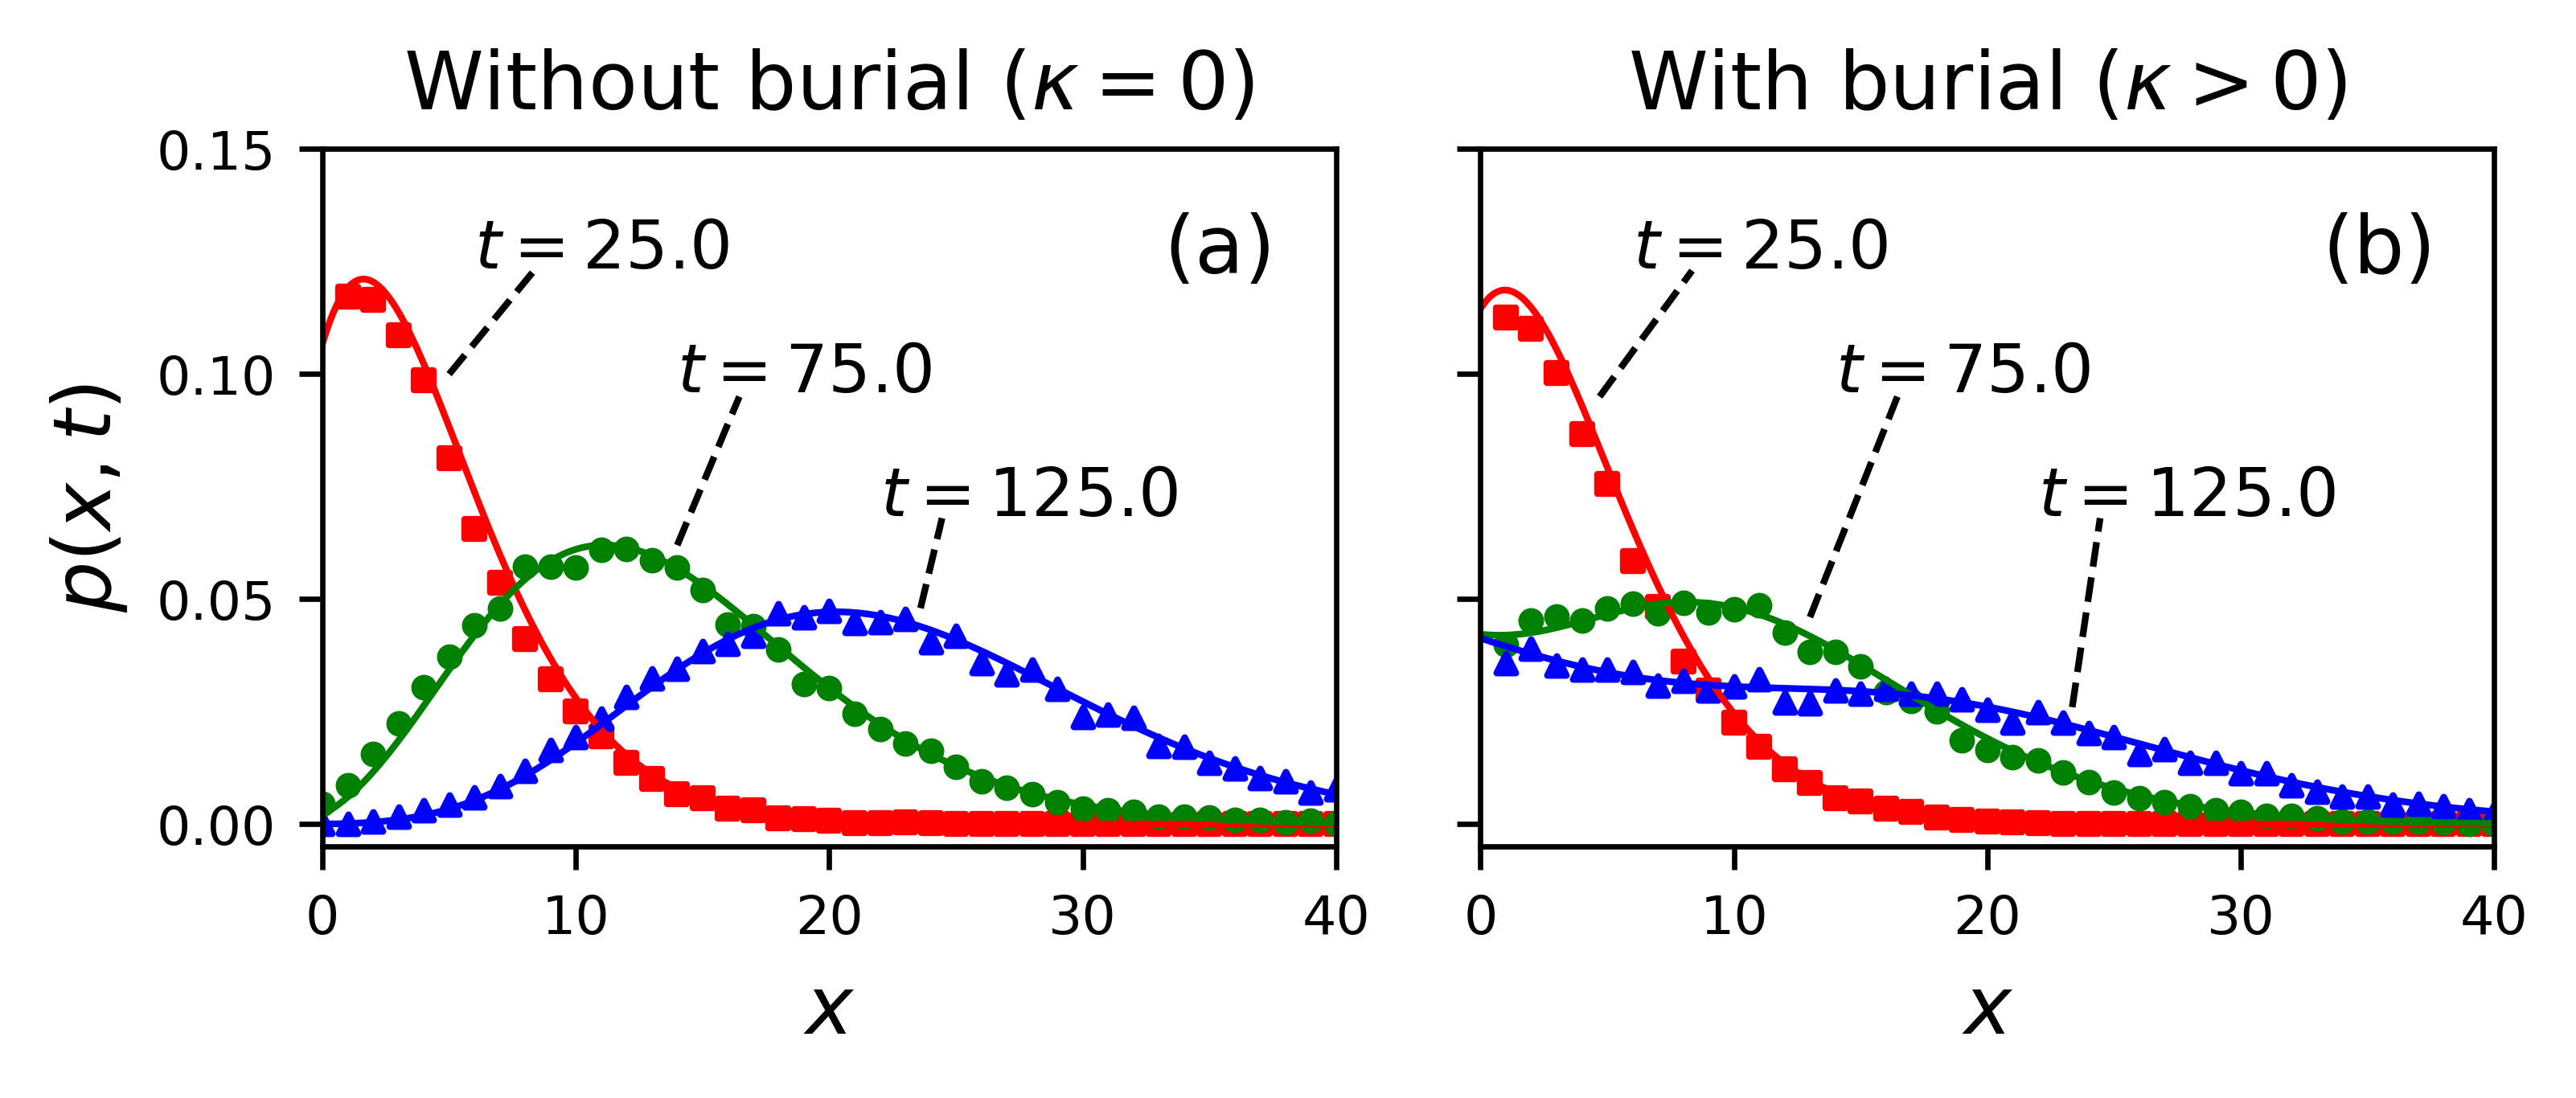
\includegraphics[width=\linewidth,keepaspectratio]{./figures/pdf-plot.png}
	\caption{Joint distributions for a grain to be at position $x$ at time $t$ are displayed for the choice $k_1=0.1$, $k_2=1.0$, $v=2.0$. Grains are considered initially at rest ($\theta_1=1$, $\theta_2=0$). The solid lines are the analytical distribution in equation (\ref{eq:pdf}), while the points are simulation results to show mathematical correctness. Colors pertain to different times. Units are unspecified, since our aim is to demonstrate the general characteristics of $p(x,t)$. Panel (a) shows the case $\kappa=0$ -- the absence of burial.
		In this case, the joint distribution tends toward Gaussian at large times \citep[e.g.,][]{Einstein1937,Lisle1998}. Panel (b) shows the case when grains have rate $\kappa = 0.01$ to become buried while resting.
		Because of burial, the joint distribution tends toward a more uniform distribution than Gaussian. This shows a redistribution of probability to smaller values of $x$ due to the burial process \citep[cf.,][]{Wu2019}. The redistribution is encoded mathematically by the Marcum Q-function terms in equation  (\ref{eq:pdf}). A similar tendency is seen in field studies of tracer dispersion in gravel bed rivers \citep[e.g.,][]{Hassan1994}.}
	\label{fig:pdfs}
\end{figure}

% solution for case theta_1=1: distribution function
Using the propagators (\ref{eq:prop1}-\ref{eq:prop2}) and this transform calculus, the joint distribution $p(x,t)$ is derived in appendix \ref{sec:appendixA}, while the moments $\bra x \ket$ and $\bra x^2 \ket$ and ultimately the variance of position $\sigma_x^2(t)$ are derived in appendix \ref{sec:appendixB}. With the shorthand notations $\xi = k_2 x/v$, $\tau = k_1(t-x/v)$, and $\Omega = (\kappa+k_1)/k_1$ \citep[cf.,][]{Lisle1998}, the joint distribution to find a grain at position $x$ at time $t$ is 
\begin{multline}
p(x,t) = \theta_1\mathcal{H}(\xi)\mathcal{H}(\tau)\Big[1-\frac{k_1}{\kappa+k_1}\Big(1-e^{-(\kappa+k_1)t}\Big)\Big]\delta(x) \\ + \frac{1}{v}e^{-\Omega \tau - \xi}\mathcal{H}(\xi)\mathcal{H}(\tau)\Big(\theta_1\Big[k_1\mathcal{I}_0\big(2\sqrt{\xi\tau}\big) + k_2\sqrt{\frac{\tau}{\xi}}\mathcal{I}_1\big(2\sqrt{\xi\tau}\big)\Big] \\ + \theta_2\Big[k_1\delta(\tau) + k_2 \mathcal{I}_0\big(2\sqrt{\xi\tau}\big)+k_1 \sqrt{\frac{\xi}{\tau}}\mathcal{I}_1\big(2\sqrt{\xi\tau}\big)\Big]\Big) \\
+ \frac{1}{v}\frac{\kappa k_2}{\kappa + k_1}e^{-\kappa \xi/(\kappa + k_1)}\mathcal{H}(\xi)\mathcal{H}(\tau)\Big[(\theta_1/\Omega)\mathcal{P}_2(\xi/\Omega,\Omega\tau) + \theta_2 \mathcal{P}_1(\xi/\Omega,\Omega\tau)\Big].
\label{eq:pdf}
\end{multline}
$\mathcal{H}$ is the Heaviside step function and we use the convention $\mathcal{H}(0)=1$.
The $\mathcal{I}_\nu$ are modified Bessel functions of the first kind, and the $\mathcal{P}_\mu$ are generalized Marcum Q-functions defined by $\mathcal{P}_\mu(x,y) = \int_0^y e^{-z-x}(z/x)^{(\mu-1)/2}\mathcal{I}_{\mu-1}(2\sqrt{xz})dz $ \citep{Temme1996}. Modified Bessel functions are common in one-dimensional diffusion problems \citep[e.g.,][]{Einstein1937,Giddings1955,Daly2010}. 

The Marcum Q-functions are convolutions between modified Bessel functions and decaying exponentials. They were originally devised in relation to radar detection theory \citep{Marcum1960}. 
Conceptually, the Q-functions emerge in our context from the sediment burial process. According to our assumptions, resting grains can become buried in some interval of time with an exponential probability. Meanwhile, the probability that grains are resting follows a modified Bessel distribution \citep[e.g.,][]{Einstein1937,Lisle1998}.
As a result, the probability that sediment is resting and becomes buried involves the convolution structure of the Marcum Q-functions.
Consistent with this interpretation, terms involving these convolutions vanish when the burial rate is taken to zero $(\kappa \rightarrow 0)$.
Figure \ref{fig:pdfs} depicts the distribution (\ref{eq:pdf}) alongside simulations generated by a direct method based on evaluating the cumulative transition probabilities between states on a small timestep \citep[cf.,][]{Barik2006}. A link to the simulation code, which includes descriptive comments, is available in the acknowledgments.



% solution for theta_1=1: moments
 The first two moments and the positional variance are derived in appendix \ref{sec:appendixB}.
The moments are
\begin{align}
\bra x(t) \ket &= A_1 e^{(b-a)t}+B_1e^{-(a+b)t}+C_1, \label{eq:mean}\\
\bra x^2(t) \ket &= A_2(t)e^{(b-a)t}+B_2(t)e^{-(a+b)t}+C_2. \label{eq:second}
\end{align}
In these equations, $a = (\kappa + k_1+k_2)/2$ and $b = \sqrt{a^2-\kappa k_2}$ are effective rates having dimensions of inverse time.
The $A_i$, $B_i$, and $C_i$ are polynomials available in table \ref{table:params}.
The variance is
\be \sigma_x^2(t) = A(t)e^{(b-a)t} + B(t)e^{-(a+b)t} + C(t). \label{eq:var}\ee
$A, B,$ and $C$ are transcendental functions available in table \ref{table:params}.
This equation represents the scale dependence of bedload diffusion for sediment gradually undergoing burial.
\begin{table}[!h]
	\centering
	\caption{Polynomials and transcendental functions used in the expressions of the mean (\ref{eq:mean}), second moment (\ref{eq:second}) and variance (\ref{eq:var}) of bedload tracers.}
	\label{table:params}
	\begin{tabular}{c}
		\toprule
		$\begin{aligned}[t]
		&A_1 = \frac{v}{2b}\big[\theta_2+\frac{k_1+\theta_2\kappa}{b-a}\big] \\
		&B_1 = -\frac{v}{2b}\big[\theta_2-\frac{k_1+\theta_2 \kappa}{a+b}\big] \\
		&C_1 =  -\frac{v}{2b}\big[\frac{k_1+\theta_2 \kappa}{b-a}+\frac{k_1+\theta_2 \kappa}{a+b}\big]\\
		&A_2(t) = \frac{v^2}{2b^3}\Big[(bt-1)[k_1+\theta_2(2\kappa + k_1 + b-a)]+\theta_2b \\
		&\hspace{3cm} + \frac{(\kappa+k_1)(\theta_2\kappa+k_1)}{(b-a)^2}[(bt-1)(b-a)-b]\Big]\\
		&B_2(t) = \frac{v^2}{2b^3}\Big[(bt+1)[k_1 + \theta_2(2\kappa+k_1-a-b)]+\theta_2b\\
		&\hspace{3cm} -\frac{(\kappa+k_1)(\theta_2\kappa+k_1)}{(a+b)^2}[(bt+1)(a+b)+b]\Big]\\
		&C_2 = \frac{v^2}{2b^3}(\kappa+k_1)(\theta_2 \kappa + k_1)\Big[\frac{2b-a}{(b-a)^2}+\frac{a+2b}{(a+b)^2}\Big]\\
		&A(t) = A_2(t)-2A_1C_1 - A_1^2\exp[(b-a)t]\\
		&B(t) = B_2(t)-2B_1C_1 - B_1^2\exp[-(a+b)t]\\
		&C(t) = C_2-C_1^2-2A_1B_1\exp[-2at]\\			
		\end{aligned}$\\
		\bottomrule
	\end{tabular}
\end{table}

The positional variance is plotted in figure \ref{fig:var} for conditions $\theta_1=1$ and $k_2\gg k_1 \gg \kappa$.
We interpret ``$\gg$'' to mean ``of at least an order of magnitude greater''.
These conditions mean that all grains are initially at rest \citep[cf.,][]{Wu2019}, motion intervals are typically much shorter than rests \citep[cf.,][]{Einstein1937}, and sediment burial requires a much longer time than typical rests.
We concentrate on these conditions in this paper as they are most relevant to bedload diffusion in gravel-bed rivers, where sediment transport is typically rarefied and intermittent, and the burial process is relatively slow compared to surface resting times \citep[e.g.,][]{Ferguson2002,Hassan1994}.
Figure \ref{fig:var} demonstrates that under these conditions the variance (\ref{eq:var}) shows three ranges of bedload diffusion each having approximate power law scaling ($\sigma_x^2 \propto t^\gamma$), followed by a fourth range with no diffusion ($\sigma_x^2 = \text{const}$). We associate the first three ranges with the local, intermediate, and global ranges proposed by \citet{Nikora2001a,Nikora2002}, and identify the fourth range as resulting from the eventual burial of all sediment grains.
We suggest to call the fourth range geomorphic, since any further transport in this range can occur only if scour exposes buried grains to the flow \citep[cf.,][]{Nakagawa1980,Voepel2013,Martin2014}.
Using this terminology, we summarize when $k_2\gg k_1 \gg \kappa$ and $\theta_1=1$, the variance in equation (\ref{eq:var}) expresses four scaling ranges: local, intermediate, and global, and geomorphic.
We emphasize only the first three of these ranges are diffusive.

\section{Discussion}
\label{sec:discussion}
\begin{figure}[t]	
	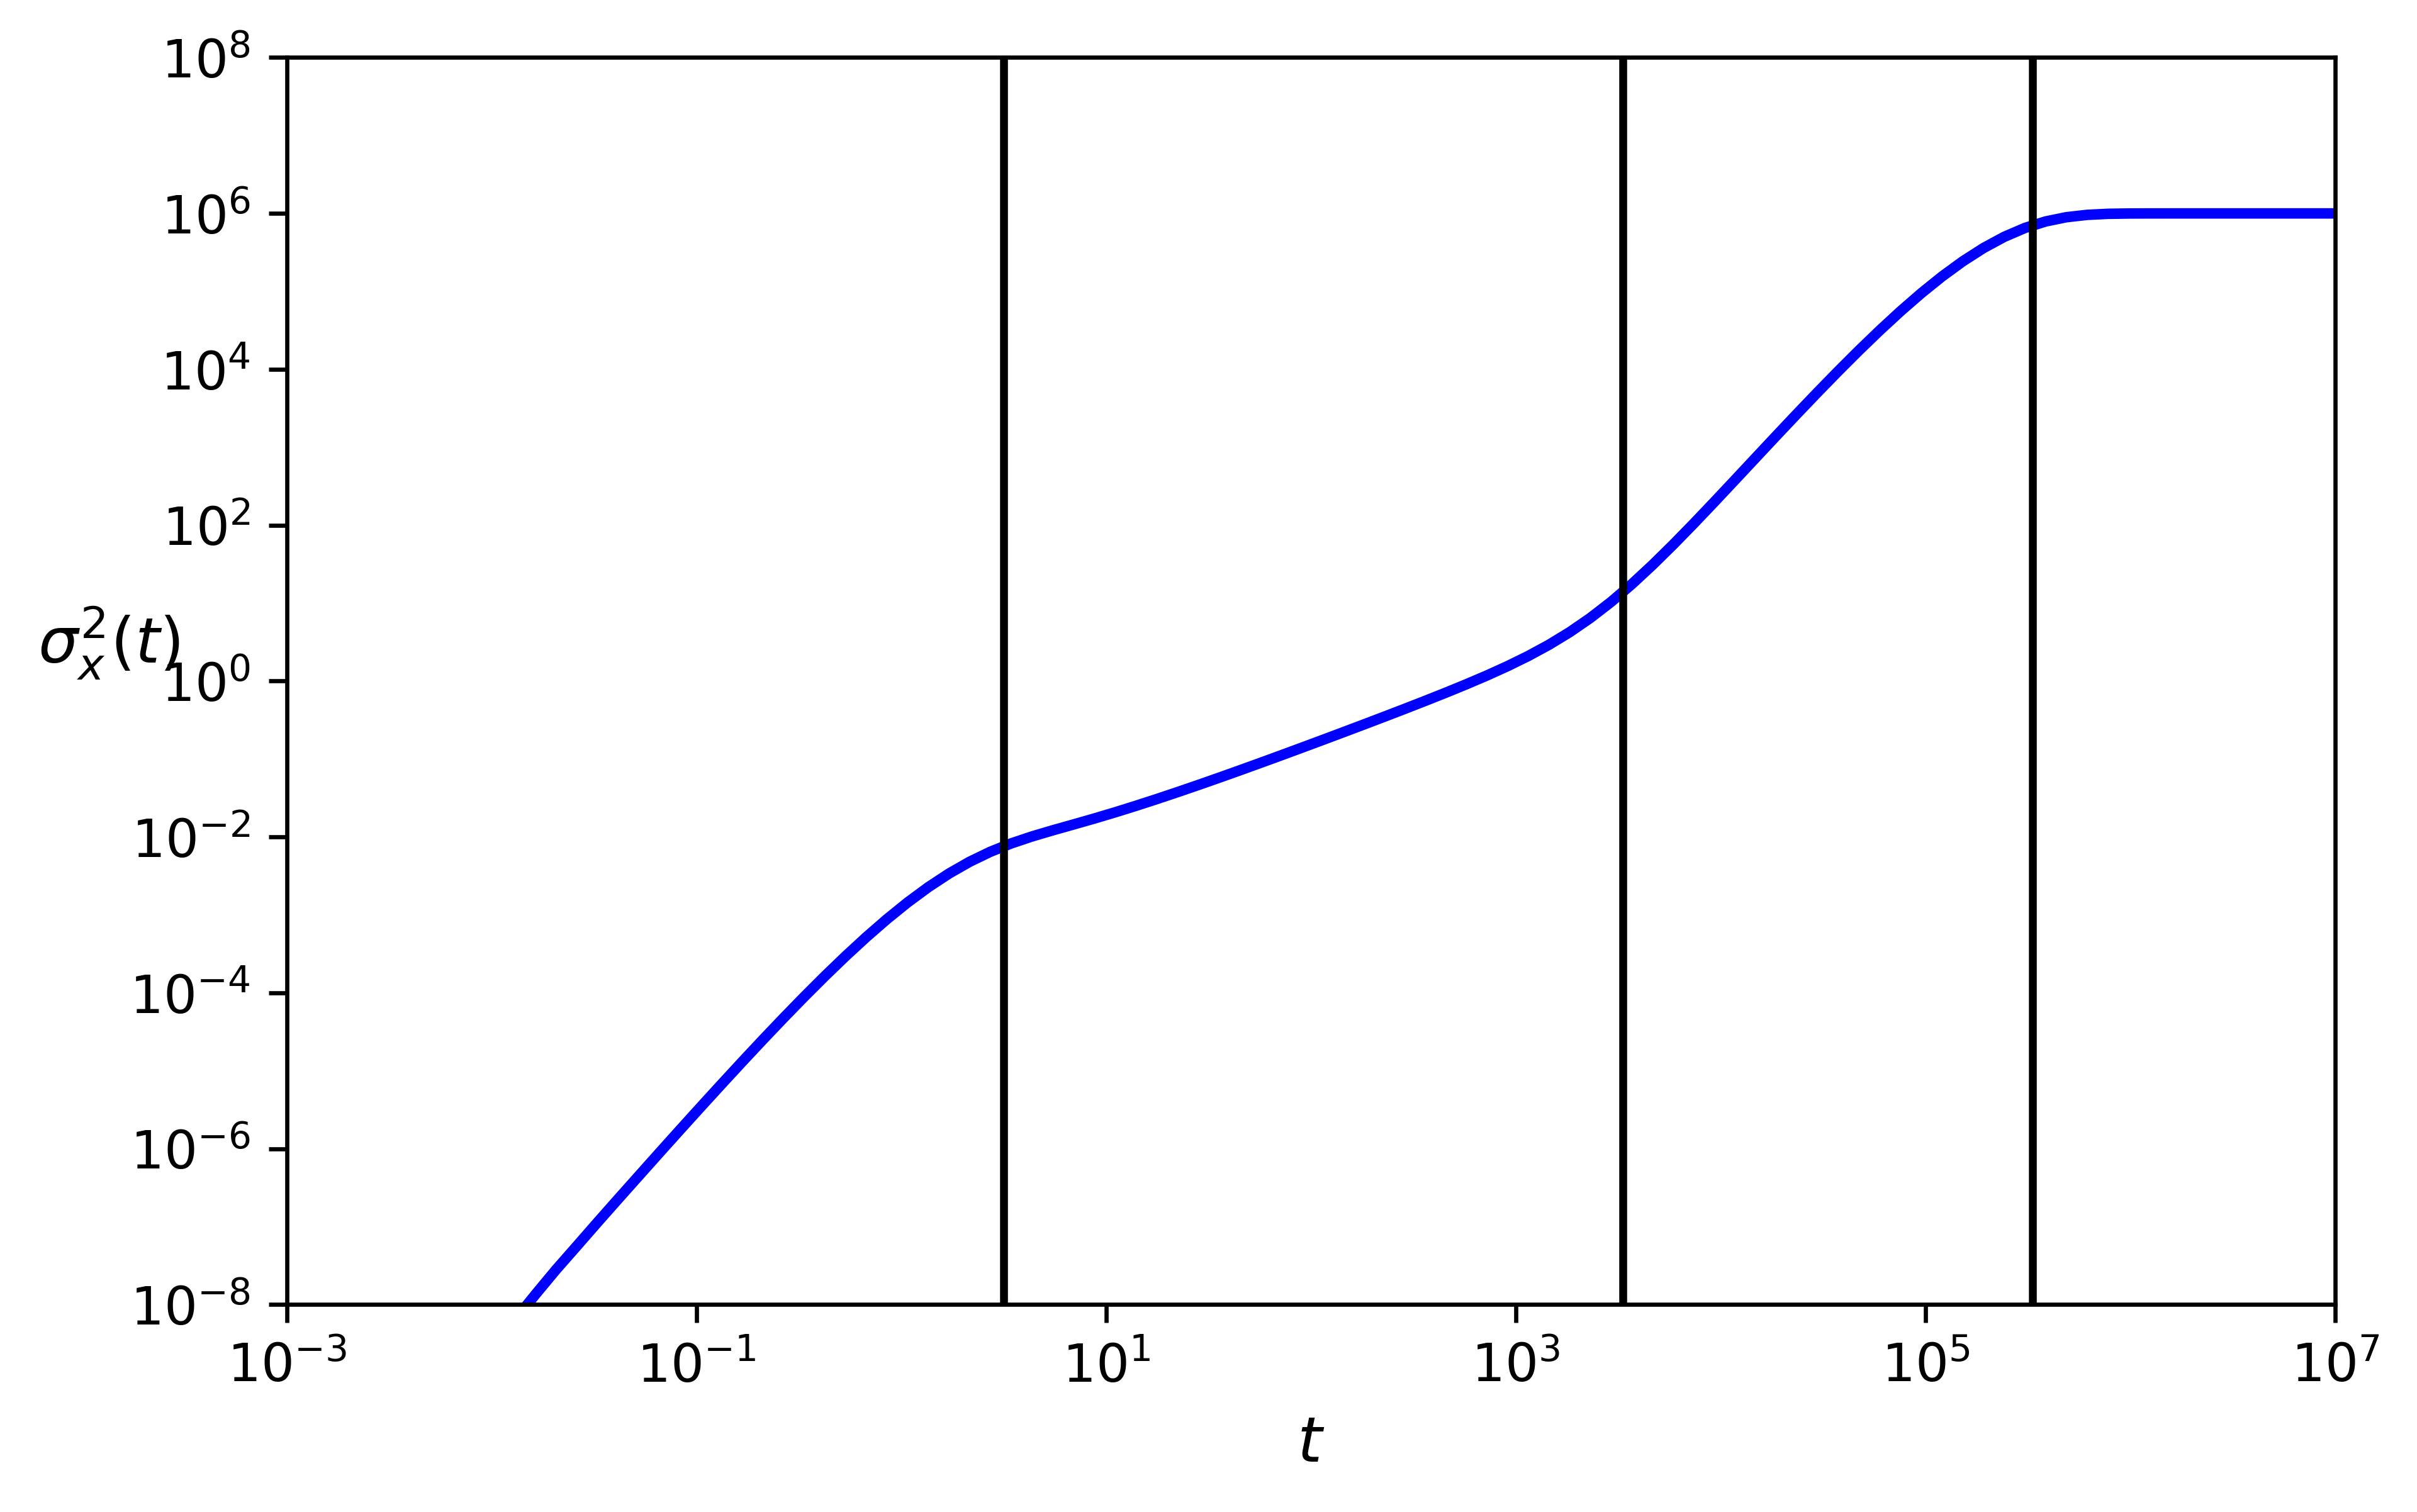
\includegraphics[width=\linewidth,keepaspectratio]{./figures/diffusion.png}
	\caption{The variance equation (\ref{eq:var}) is plotted for the parameters $1/k_2 = 1.5$s, $1/k_1 = 30.0$s, and $v=0.1$m/s. These values are comparable to laboratory flume experiments transporting small ($\sim 5$mm) gravels \citep[cf.,][]{Lajeunesse2010,Martin2012}. The timescale of burial is set to $1/\kappa = 7200.0$s (two hours), and the initial condition is rest ($\theta_1=1$). The solid line is equation (\ref{eq:var}) while the points are directly simulated. When $k_2\gg k_1 \gg \kappa$, as as is the case in this plot, there are four distinct scaling ranges of $\sigma_x^2$: local, intermediate, global, and geomorphic. Within each range, a slope key is added to demonstrate the scaling $\sigma_x^2 \propto t^\gamma$. There are three crossovers between these ranges, denoted on the figure by vertical lines. Crossover times $T_L$, $T_I$, and $T_G$ are indicated at the bottom of the plot. They are given in equations (\ref{eq:TL}-\ref{eq:TG}) in terms of the model's input parameters. }
	\label{fig:var}
\end{figure}

The model we've presented involves four parameters. These are the characteristic velocity $v$ of moving sediment and three key timescales: $1/k_2$, $1/k_1$, and $1/\kappa$.
The timescales represent the mean duration of motion, the mean duration of rest, and the mean duration of rest before burial occurs.
As shown in figure \ref{fig:var}, scaling laws $\sigma_x^2 \propto t^\gamma$ approximately characterize the diffusion in each scaling range.
The exponents $\gamma$ in each range result from competition between different terms in equation (\ref{eq:var}).
Between these ranges, there are crossover regions where the scaling is not a simple power law.
Because these crossover regions are relatively narrow, we can approximately characterize them with crossover times $T_L$, $T_I$, and $T_G$.
These times partition the diffusion ranges into $0< t < T_L$ (local), $T_L < t < T_I$ (intermediate), $T_I < t < T_G$ (global), and $T_G < t$ (geomorphic). 
Figure \ref{fig:var} depicts these crossover times as vertical lines.
To understand the scale dependence expressed by the bedload variance in equation (\ref{eq:var}), we need to determine the exponents $\gamma$ of each range and relate the crossover times $T_L$, $T_I$, and $T_G$ between diffusion ranges to the model parameters $v$, $k_1$, $k_2$, and $\kappa$.

% now we figure out what the exponents are 
We determine the diffusion exponents $\gamma$ in the local, intermediate, and global ranges using two limiting cases of equation (\ref{eq:var}): (1) $t\ll 1/\kappa$, and (2) $1/k_2 \rightarrow 0$ while $vk_2 = \text{const}$.
Limit (1) corresponds to times so short a negligible amount of sediment burial has occurred, while limit (2) corresponds to times so long a motion interval appears as an instantaneous step having mean step length $l=vk_2$.
We evaluate these limits in appendix \ref{sec:appendixC} and obtain the diffusion exponents.
Local range diffusion has exponent $2 \leq \gamma \leq 3$ depending on the initial conditions $\theta_1$ and $\theta_2$.
When the initial conditions are pure, meaning one of the $\theta_i$ is zero, the local exponent is $\gamma=3$.
When grains start in a mixture of motion and rest states, meaning neither $\theta_i$ is zero, the local exponent is $\gamma=2$.
Intermediate range diffusion always has exponent $\gamma=1$, agreeing with classic flume experiments \citep[e.g.,][]{Einstein1937,Yano1969a,Nakagawa1976}.
Finally, global range diffusion has exponent $1 < \gamma < 3$ depending on the ratio $k_1/\kappa$.
In the extreme case $k_1/\kappa \approx 0 $, we find normal diffusion $\sigma_x^2 \propto t$. 
However, in the opposite extreme $k_1/\kappa \rightarrow \infty$, we find  super-diffusion $\sigma_x^2 \propto t^3$.
For general ratios $\kappa/k_1$, the global exponent lies between these extremes.
For example, when $k_1/\kappa \approx 240$ as in figure \ref{fig:var}, the global range exponent is $\gamma \approx 2.2$. 
We surmise when the model parameters satisfy $k_2\gg k_1 \gg \kappa$ meaning all three diffusion ranges exist, the variance (\ref{eq:var}) implies local range super-diffusion with exponent depending on the $\theta_i$, intermediate range normal diffusion with no dependence on model parameters, and global range super-diffusion with exponent depending on the ratio $k_1/\kappa$.
Finally, the model supports a geomorphic range of no diffusion ($\gamma=0$) associated with the eventual and long term burial of all sediment grains.

Each of the three crossover times relates to a physical process affecting a population of grains.
Exchange between motion and rest states induces the local/intermediate crossover, the onset of sediment burial induces the intermediate/global crossover, and the completion of sediment burial induces the global/geomorphic crossover.
Each process admits two characteristic times, and we formulate the crossover times heuristically as geometric averages of these characteristic times:
\begin{alignat}{2}
&T_L &&= \sqrt{\frac{1}{k_1}\frac{1}{k_2}}, \label{eq:TL}\\
&T_I &&= \sqrt{\frac{1}{k_1}\frac{1}{\kappa}},\label{eq:TI}\\
&T_G &&= \sqrt{\frac{1}{\kappa}\frac{k_1+k_2}{\kappa k_1}} \label{eq:TG}.
\end{alignat}
Figure \ref{fig:var} depicts these relationships as dashed vertical lines.
The times $1/k_1$ and $1/k_2$ characterize exchanges between motion and rest, while $1/k_1$ and $1/\kappa$ characterize the onset of burial originating from grains buried in their first resting sojourns.
Equations (\ref{eq:TL}) and (\ref{eq:TI}) mix these paired times.
The completion of sediment burial and its characteristic timescales originate from the last grains to bury.
In one extreme, all grains rest on the surface, meaning the last grains bury around $1/\kappa$; while in another, a fraction of grains remains in motion for a long time evading burial.
By analogy to the mobile-immobile model of \citet{Ancey2006}, we reason that a fraction $k_1/(k_1+k_2)$ of the free population will be in motion and evading burial at long timescales, and for this fraction we propose an effective trapping rate $\kappa k_1/(k_1+k_2)$.
Equation (\ref{eq:TG}) mixes the reciprocal of this effective rate with $1/\kappa$.
We tested formulas (\ref{eq:TL}-\ref{eq:TG}) for many parameter choices and conclude they adequately represent the crossover locations between diffusion regimes provided the parameters satisfy $k_2\gg k_1 \gg \kappa$ and grains start from rest ($\theta_1=1$).
However, starting grains from motion ($\theta_2=1$) widens the crossover region between local and intermediate ranges, meaning equation (\ref{eq:TL}) loses representative power; while setting relatively very large values of $k_2$ widens the crossover region between global and geomorphic ranges, meaning equation (\ref{eq:TG}) loses representative power.
Ultimately, we emphasize the representation of finite width crossover regions by crossover times is an idealization, so we propose equations (\ref{eq:TL}-\ref{eq:TG}) as heuristics. 
These relations provide useful divisions between the bedload diffusion scaling ranges.

Our four range bedload diffusion model reduces to earlier works through the two simplified limits previously leveraged to extract the scaling exponents $\gamma$ and explored in appendix \ref{sec:appendixC}.
Limit (1) implies the model developed by \citet{Lisle1998} to describe soil transport within a sheet flow, while limit (2) implies the model developed by \citet{Wu2019} to describe bedload transport with burial.
Either of these cases further simplifies to the classic results of \citet{Einstein1937} and his early followers \citep[e.g.,][]{Hubbell1964, Nakagawa1976, Yano1969} that predict a single range of normal diffusion.
\citet{Lisle1998} generalized the Einstein model to include a finite velocity and duration of motion in place of instantaneous steps, and they derived two ranges of diffusion -- super-diffusive and normal.
\citet{Wu2019} developed an active layer formulation of bedload transport where grains are transferred from the active layer (surface) to the substrate layer (burial) at a constant rate.
They simplified the problem by interpreting motions as instantaneous steps, and they derived two ranges of diffusion -- normal and super-diffusive.
Our model ultimately extends these two works and re-frames them in the formalism of CTRWs \citep[e.g.,][]{Weiss1994} that was implicitly applied by \citet{Einstein1937}.

We offer several implications of our model for bedload diffusion studies in gravel bed streams.
First, our model confines the valid range of scale independent models such as the advection-diffusion equation \citep[e.g.,][]{Bradley2010} and the Einstein model \citep[e.g.,][]{Martin2012} for practical applications such as contaminant transport \citep[e.g][]{Malmon2005,Macklin2006} and aquatic habitat restoration \citep[e.g.,][]{Gaeuman2017}.
We can conclude when the observation timescale satisfies $T_L<t<T_I$, with $T_L$ and $T_I$ given by equations (\ref{eq:TL}) and (\ref{eq:TI}), we expect normal bedload diffusion $\sigma_x^2 = D_d t$.
Second, the model links bedload transport understanding across scales. 
In practice, we might measure sediment diffusion within a channel on one timescale with intent to apply our knowledge at smaller or larger timescales; usually, experimental limitations constrain the measurement timescale.
For example, we could determine $k_1$ and $k_2$ by measuring the virtual velocity and diffusivity of sediment tracers in the intermediate range \citep[e.g.,][]{Einstein1937,Yano1969a,Nakagawa1976}.
With an estimate of the trapping rate $\kappa$, equation (\ref{eq:var}) provides diffusion characteristics of the global range $T_I<t<T_G$ which is more difficult to study experimentally.

To describe the scale dependence of bedload diffusion, we extended the original Einstein model by building up ideas from condensed matter physics.
Along the way, we incorporated two simplifying assumptions that deserve further research attention. 
First, we treated sediment burial as a quasi permanent condition; and second, we implicitly assumed burial is the only process trapping grains in river channels.
In actuality, burial is a temporary condition linked to scour and fill of the sedimentary bed \citep{Hassan1994,Voepel2013,Martin2014}, and field experiments show other processes trapping sediment.
For example, grains can become stranded on bars \citep{Ferguson2002,Bradley2017} and embedded in stabilizing structures such as steps or clusters \citep[e.g.][]{Church1998,Hassan2008}.
In principle, the multi state CTRW framework we developed here can describe bedload diffusion with multiple trapping processes by simply adding more states, and it can handle impermanent sojourns in these states by specifying propagators for them.
Unfortunately, we currently lack the experimental knowledge to specify these propagators, since trapping rates and durations are poorly understood in association with particular processes.
For example, recent experiments have attributed resting times to any immobile sediment, and this is known to imply heavy-tailed sediment resting time distributions \citep[e.g.,][]{Olinde2015,Bradley2017}.
However, very few studies have resolved immobile times of sediment while identifying their underlying mechanism \citep[e.g.,][]{Martin2014}.
We propose experiments to determine the rates and durations of specific bedload trapping processes as important topics for further study.
A first step might be to measure the burial rate $\kappa$ we applied in this paper; in principle, this could be discerned by timing the period required for tagged surface grains to become buried in flume experiments.
Once better understanding of the rates and durations of sediment trapping processes is in place, generalizations built from the framework we've presented in this paper should better predict bedload diffusion on the global and geomorphic scales.


\section{Conclusion}
\label{sec:conclusion}
We developed a random walk model with alternating mobile and immobile states and a possibility of trapping from the immobile state, and we used it to describe sediment transporting through a river channel as it gradually becomes buried.
To our knowledge, this is the first analytical description of bedload diffusion across the local, intermediate, and global timescales introduced by \citet{Nikora2001a}.
Pushing the ideas of Nikora et al. somewhat further, we proposed a geomorphic range to describe diffusion characteristics at timescales larger than the global range.
At base level, our model demonstrates the required components for three bedload diffusion ranges: (1) the duration of sediment motions, (2) mobile-immobile switching, and (3) a sediment trapping process.
A next step is to incorporate the bed scour process that re-exposes buried sediment to better understand the global and geomorphic ranges.
Ultimately, we emphasize the multi state random walk formalism used in this paper implicitly underlies most existing bedload diffusion models, and we believe it will readily accommodate efforts to include more physical processes into Einstein's research paradigm.

\appendix

\section{Calculation of the distribution function}
\label{sec:appendixA}
Double transforming (\ref{eq:x}-\ref{eq:y}) using the definition (\ref{eq:doubletransform}) gives

\begin{alignat}{2}
&\tom_{1T}(\eta,s) &&= \theta_1 \tg_1(\eta,s) + \tom_2(\eta,s)\tg_1(\eta,s)-\tom_{1F}(\eta,s),\\
&\tom_{1F}(\eta,s) &&= \theta_1\tg_1(\eta,s+\kappa) + \tom_2(\eta,s)\tg_1(\eta,s+\kappa),\\
&\tom_2(\eta,s) &&= \theta_2 \tg_2(\eta,s) + \tom_{1F}(\eta,s)\tg_2(\eta,s).
\end{alignat}
This algebraic system solves for 
\begin{alignat}{2}
&\tom_{1T}(\eta,s) &&= \frac{\theta_1 + \theta_2 \tg_2(\eta,s)}{1-\tg_1(\eta,s+\kappa)\tg_2(\eta,s)}\big\{\tg_1(\eta,s)-\tg_1(\eta,s+\kappa) \big\}, \label{eq:A} \\
&\tom_{1F}(\eta,s) &&= \frac{\theta_1 + \theta_2 \tg_2(\eta,s)}{1-\tg_1(\eta,s+\kappa)\tg_2(\eta,s)}\tg_1(\eta,s+\kappa),\\
&\tom_{2}(\eta,s) &&= \frac{\theta_2 + \theta_1 \tg_1(\eta,s+\kappa)}{1-\tg_1(\eta,s+\kappa)\tg_2(\eta,s)}\tg_2(\eta,s). 
\end{alignat}
Double transforming (\ref{eq:b}-\ref{eq:z}) gives
\begin{align}
\tp_0(\eta,s) &= \frac{1}{s}\tom_{1T}(\eta,s),\\
\tp_1(\eta,s) &= \theta_1 \tG_1(\eta,s) + \tom_2(\eta,s) \tG_1(\eta,s),\\
\tp_2(\eta,s) &= \theta_2 \tG_2(\eta,s) + \tom_{1F}(\eta,s)\tG_2(\eta,s).\label{eq:Z}
\end{align}
The total probability is $p(x,t) = p_0(x,t) + p_1(x,t) + p_2(x,t)$. Using equations (\ref{eq:A}-\ref{eq:Z}) this becomes, in the double Laplace representation, 
\begin{multline}
\tp(\eta,s) = \frac{1}{s}\frac{\theta_1 + \theta_2 \tg_2(\eta,s)}{1-\tg_1(\eta,s+\kappa)\tg_2(\eta,s)}\big\{\tg_1(\eta,s)-\tg_1(\eta,s+\kappa) \big\} \\
+\frac{\theta_1\big[\tG_1(\eta,s) + \tg_1(\eta,s+\kappa)\tG_2(\eta,s)\big]+ \theta_2\big[\tG_2(\eta,s) + \tg_2(\eta,s)\tG_1(\eta,s)\big]}{1-\tg_1(\eta,s+\kappa)\tg_2(\eta,s)}. \\
\label{eq:lap}
\end{multline}
Plugging the propagators outlined in equations (\ref{eq:prop1}-\ref{eq:prop2}) into equation (\ref{eq:lap}) gives 
\be \tilde{p}(\eta,s) = \frac{1}{s}\frac{(s+\kappa + k')s  + \theta_1(s+\kappa )\eta v+ \kappa k_2}{(s+\kappa+k_1)\eta v+(s+\kappa+k')s + \kappa k_2}.\label{eq:nicedist}\ee
In this equation, $k'=k_1+k_2$, and we have used the normalization requirement of the initial probabilities: $\theta_1 + \theta_2 = 1.$
The double inverse transform of this equation provides the distribution $p(x,t)$.
We invert the transform over $\eta$ first.
Using the results 15.103 (transform of exponential), 15.123 (transform of derivative), and 15.141 (transform of Dirac delta function) from \citet{Arfken1985} provides 
\begin{multline} \tp(x,s) = \theta_1 \frac{s+\kappa}{s(s+\kappa + k_1)}\delta(x) + \frac{1}{v} \Big(\frac{(s+\kappa+k')s+\kappa k_2}{s(s+\kappa+k_1)} \\- \frac{\theta_1(s+\kappa)[s(s+\kappa+k_1)+\kappa k_2]}{s(s+\kappa+k_1)^2}\Big)
\exp\Big[-\frac{(s+\kappa+k')s+\kappa k_2}{s+\kappa+k_1}\frac{x}{v}\Big].\end{multline}
Inverting the remaining transform over $s$, applying results 15.152 (substitution), 15.164 (translation), and 15.175 (transform of $te^{kt}$) from \citet{Arfken1985}, and defining the shorthand notations $\tau = k_1(t-x/v)$, $\xi = k_2 x/v$, and $\Omega = (\kappa + k_1)/k_1$, gives the simpler form 
\begin{multline}
p(x,t) = \theta_1\Big[1-\frac{k_1}{\kappa + k_1}\big(1-e^{-(\kappa + k_1)t}\big)\Big]\delta(x) + \frac{1}{v}\exp[\Omega \tau - \xi]\\
\times \El^{-1}\Big\{\Big( \theta_2 + \frac{\theta_1k_1+\theta_2 k_2}{s}+\frac{\theta_1k_1k_2}{s^2} + \frac{\theta_2\kappa k_2}{s(s-\kappa-k_1)} + \frac{\theta_1\kappa k_1 k_2}{s^2(s-\kappa-k_1)}\Big)\\
\times\exp\big[\frac{k_1 \xi}{s}\big];\tau/k_1\Big\}.
\end{multline}
Using entries 2.2.2.1, 2.2.2.8, and 1.1.1.13 from \citet{Prudnikov1992a} in conjunction with the definition of the Marcum Q-function $ \mathcal{P}_\mu(x,t)$ \citep[e.g.,][]{Temme1996}, and inserting the Heaviside functions to account for the fact that grains can neither travel backwards nor at speeds exceeding $v$, we finally arrive at equation (\ref{eq:pdf}) for the joint distribution $p(x,t)$.

\section{Calculation of the moments}
\label{sec:appendixB}
We compute the first two moments of position $x$ and ultimately its variance using equation (\ref{eq:momenttrick}). The first two derivatives of the double Laplace transformed distribution (\ref{eq:nicedist}) are
\be \partial_\eta \tp(\eta,s) = -v \frac{1}{s}\frac{[(s+\kappa + k')s + \kappa k_2][\theta_2(s+\kappa) + k_1]}{[\eta v(s+\kappa +k_1) + (s+ \kappa + k')s+\kappa k_2]^2},\ee
\be \partial_\eta^2 \tp(\eta,s) = 2v^2 \frac{1}{s} \frac{(s+\kappa+k_1)[(s+\kappa + k')s+\kappa k_2][\theta_2(s+\kappa) + k_1]}{[\eta v(s+\kappa + k_1) + (s+\kappa + k')s+ \kappa k_2]^3}.\ee
Evaluating these at $\eta=0$ and applying equation (\ref{eq:momenttrick}) provides the Laplace transformed moments
\be  \frac{\bra\tilde{x}(s)\ket} {v} = \frac{1}{s}\frac{\theta_2(s+\kappa)+k_1}{(s+\kappa+k')s+\kappa k_2} = \frac{1}{s} \frac{\theta_2(s+\kappa)+k_1}{(s+a+b)(s+a-b)}\label{eq:lapmean},\ee
\be \frac{\bra \tilde{x}^2(s) \ket}{2v^2} = \frac{1}{s} \frac{(s+\kappa+k_1)(\theta_2(s+\kappa)+k_1)}{[(s+\kappa+k')s+\kappa k_2]^2}=  \frac{1}{s}\frac{(s+\kappa+k_1)(\theta_2(s+\kappa)+k_1)}{(s+a+b)^2(s+a-b)^2}.\label{eq:lapsecondmom}\ee
The parameters $a= (\kappa+k')/2$ and $b^2 = a^2 -\kappa k_2$ were introduced to factorize the denominators.
These equations can be inverted using the properties 15.164 (translation), 15.11.1 (integration), and 15.123 (differentiation) from  \citet{Arfken1985} after expansion in partial fractions.
For the mean, the calculation is
\begin{align}
\frac{2b}{v}\bra x \ket &= \big[\theta_2 + (k_1+\theta_2 \kappa)\int_0^t dt\big]\El^{-1}\Big\{ \frac{1}{s+a-b}-\frac{1}{s+a+b};t\Big\}\\
&= \Big[\theta_2 + \frac{k_1+\theta_2\kappa}{b-a}\Big]e^{(b-a)t} - \Big[\theta_2 - \frac{k_1+\theta_2\kappa}{a+b}\Big]e^{-(a+b)t} - \Big[\frac{k_1+\theta_2\kappa}{b-a} + \frac{k_1+\theta_2\kappa}{a+b}\Big].
\end{align}
This equation rearranges to (\ref{eq:mean}).
The second moment (\ref{eq:lapsecondmom}) is 
\begin{multline}
\frac{2b^2}{v^2}\bra x^2 \ket = \Big[\theta_2(\delta(t) + \partial_t) + (\theta_2(2\kappa + k_1)+k_1) + (\kappa+k_1)(\theta_2\kappa+k_1)\int_0^t dt \Big] \\
\times \El^{-1}\Big\{ \frac{1}{(s+a-b)^2} + \frac{1}{(s+a+b)^2}-\frac{1}{b(s+a-b)}+\frac{1}{b(s+a+b)};t\Big\}.
\end{multline}
This becomes 
\begin{multline}
\frac{2b^3}{v^2}\bra x^2 \ket = \Big[\theta_2\partial_t + [\theta_2(2\kappa+k_1)+k_1] + (\kappa+k_1)(\theta_2\kappa+k_1)\int_0^tdt\Big]\\
\times \Big((bt-1)e^{(b-a)t}+(bt+1)e^{-(a+b)t}\Big)
\end{multline}
which evaluates to equation (\ref{eq:second}).
$\sigma_x^2 = \bra x^2 \ket - \bra x \ket^2$ derives the variance in equation (\ref{eq:var}).

\section{Limiting behavior of the moments}
\label{sec:appendixC}

Limit (1) is $\kappa \rightarrow 0$. We take this limit in equations (\ref{eq:lapmean}) and (\ref{eq:lapsecondmom}) with initial condition $\theta_1=1$ to obtain
\begin{align}
\bra \tilde{x} \ket &= vk_1 \frac{1 }{s^2(s+k')}, \label{eq:li1}\\
\bra \tilde{x}^2 \ket &= 2v^2k_1 \frac{s+k_1}{s^3(s+k')^2}. \label{eq:li2}
\end{align}
Inverting these equations provides the variance
\be \sigma_x^2 = 2v^2\frac{k_1}{k'^4}\Big(k_1\big[\frac{1}{2} - k'te^{-k't} - \frac{1}{2} e^{-2k't}\big] + k_2\big[-2+k't + (2+k't)e^{-k't}\big]\Big).\label{eq:li}\ee
This result encodes two ranges of diffusion and can also be derived from the governing equations of the \citet{Lisle1998} model.
Expanding for small $t$ provides $\sigma_x^2(t) = v^2k_1t^3/3$ -- local range super-diffusion.
Expanding for large $t$ provides $\sigma_x^2(t) = 2v^2k_1k_2t/k'^3$ -- intermediate range normal diffusion.

We further investigate limit (1) for arbitrary initial conditions.
By applying Tauberian theorems, we assert the $ t \rightarrow 0$ variance is determined by the $s\rightarrow \infty$ limits of (\ref{eq:lapmean}) and (\ref{eq:lapsecondmom}) \citep[e.g.,][]{Weiss1994, Weeks1998}.  
Expanding these equations in powers of $1/s$ and inverting the resulting transforms gives
\begin{align} \bra x \ket &= v \theta_2 t + \frac{1}{2}v(\theta_1k_1-\theta_2k_2)t^2 + O(t^3),\\
\bra x^2 \ket &= v^2\theta_2 t^2 + \frac{1}{3}v^2(\theta_1k_1-2\theta_2k_2)t^3+ O(t^4).
\end{align}
This equation highlights the effect of initial conditions on the diffusion characteristics of the local range:
\be \sigma_x^2(t) \sim v^2\theta_1\theta_2t^2 + \frac{1}{3}v^2(\theta_1k_1+\theta_2k_2)t^3.\label{eq:init}\ee
We have taken only leading order terms for any option of $\theta_1$ and $\theta_2$.
Equation (\ref{eq:init}) shows local range exponent $\gamma=2$ when initial conditions are mixed (both are non-zero) and $\gamma=3$ when initial conditions are pure (one is zero).

Limit (2) is $1/k_2 \rightarrow 0$ and $v\rightarrow \infty$ while $v/k_2 = l$. Under this limit, equations (\ref{eq:lapmean}) and (\ref{eq:lapsecondmom}) provide
\begin{align}
\bra \tilde{x} \ket &= k_1l\frac{1}{s(s+\kappa)},\\
\bra \tilde{x}^2 \ket &= 2l^2k_1 \frac{s+\kappa+k_1}{s(s+\kappa)^2}.
\end{align}
Inverting these equations and introducing the variables $c=lk_1$ (an effective velocity) and $D_d = l^2k_1$ (a diffusivity) provides positional variance
\be \sigma_x^2(t) = \frac{2D_d(1-e^{-\kappa t})}{\kappa} + \frac{(1-e^{-2\kappa t}-2e^{-\kappa t}\kappa t)c^2}{\kappa^2}. \label{eq:wuvar}\ee
This is mathematically identical to the key result of \citet{Wu2019}.
Expanding for small $t$ provides $\sigma_x^2(t) = 2D_d t$ -- intermediate range normal diffusion, while sending $t\rightarrow \infty$ provides $\sigma_x^2 = (2D_d\kappa + c^2)/\kappa^2$ -- a constant variance in the geomorphic range.
The global range is characterized by competition between terms in equation (\ref{eq:wuvar}), and shows $2 \leq \gamma \leq 3$ depending on the ratio $k_1/\kappa$ \citep[cf.,][]{Wu2019}.
Finally, both equations (\ref{eq:li}) and (\ref{eq:wuvar}) reduce to the Einstein result $\sigma_x^2(t) = 2D_d t$ in further simplified limits.

\acknowledgments
J. Pierce acknowledges helpful exchanges with Eduardo Daly and Peter H{\"a}nggi during the early stages of this work. He would like to thank Melinda Saunders and Leonardo Golubovic for their careful guidance in mathematics through the years. M. Hassan is supported by an NSERC Discovery grant. The Python simulation code is available at \sloppy
\url{https://github.com/kevinkayaks/rw-diffu}.

\bibliography{biblio.bib}
\end{document}